% \pagebreak[4]
% \hspace*{1cm}
% \pagebreak[4]
% \hspace*{1cm}
% \pagebreak[4]
%\usepackage[round,colon,authoryear]{natbib}

\chapter{A pipeline for the analysis of TraDIS experiments, with an application to {\it Salmonella} macrophage invasion}
\label{sec:chapterPingpong}
\ifpdf
    \graphicspath{{Chapter3/Chapter3Figs/EPS/}{Chapter3/Chapter3Figs/}}
\fi

\textit{Section 3.2 describes a collaborative study with Gemma C. Langridge (Pathogen Genomics, Wellcome Trust Sanger Institute). Gemma performed all laboratory experiments described in this chapter unless otherwise noted.}

\section{Introduction}

In the previous chapter, I described the results of a study predicting and comparing the genes required for robust growth of two \textit{Salmonella} serovars in standard laboratory media. While this revealed interesting aspects of \textit{Salmonella} biology, linking these findings to \textit{Salmonella}'s infective niche in the human host is difficult. However, transposon-insertion sequencing can be used to interrogate infective conditions directly (reviewed previously in section 1.5): by comparing libraries passed through a condition of interest to control libraries, we can determine the genomic regions involved in survival in that condition. In this chapter, I describe a pipeline I have devised for the analysis of such experiments, illustrated with an experiment assaying genes required for \textit{S.} Typhi and Typhimurium invasion of (or uptake into) human macrophage. These methods have been adopted by Pathogen Informatics at the Sanger, form the basis of the current Sanger pipelines for analysis of TraDIS experiments, and are currently being used in a variety of transposon-insertion sequencing studies.

\subsection{\textit{Salmonella} interactions with macrophage}

As previously described in section 2.1, the ability to invade and survive in host cells was a major factor in the early evolution of \textit{S. enterica} subspecies \textit{enterica}; survival in macrophages in particular is known to be necessary for virulence \parencite{Fields1986}. This ability appears to have been largely driven by the acquisition of two horizontally-acquired pathogenicity islands, SPI-1 and -2. Due to the availability of a mouse model of systemic infection \parencite{Santos2001}, most of what is known about \textit{Salmonella} interactions with host cells is derived from studies of \textit{S.} Typhimurium infection.

\textit{S.} Typhimurium infections of either epithelial or phagocytic cells appear to follow broadly similar paths (\textcite{Figueira2012}, see also figure \ref{fig:SCV}). On encountering a suitable host cell, the bacterium adheres using an array of fimbrial adhesins \parencite{Baumler1996a, Velden1998}. The SPI-1 T3SS, a needle-like complex spanning the periplasm and presenting its tip to the exterior of the bacterial cell \parencite{Mueller2008}, induces membrane ruffling in the host cell through secretion of effector proteins \parencite{Zhou2001}, facilitating bacterial uptake. While use of this mechanisms is not strictly necessary for entrance to phagocytic cells such as macrophage, {\it S.} Typhimurium strains unable to induce ruffling are taken up six to ten times less efficiently than the wild-type \parencite{Monack1996}, though the entry mechanism does not ultimately affect cell fate \parencite{Rathman1997}.

Once entry has been gained to the cell, through either active invasion or phagocytic engulfment, {\it S.} Typhimurium begins expressing a second T3SS encoded by SPI-2. The effectors secreted by this T3SS allow {\it S.} Typhimurium to remodel the \textit{Salmonella} containing vacuole (SCV)\nomenclature[Z]{SCV}{\textit{Salmonella} containing vacuole}, and even modulate host immune signalling (see figure \ref{fig:SCV}). There is some controversy as to whether or not the SCV undergoes fusion with lysosomes; a recent study suggests it does, but that the activity of these lysosomes is first modulated by the SPI-2 effector SifA \parencite{McGourty2012}. Little is known about the growth conditions {\it S.} Typhimurium faces within the SCV, though transcriptomic studies suggest it is aerobic, mildly acidic, rich in gluconate, and limited in aromatic amino acids, purines, and pyrimidines \parencite{Eriksson2003, Hautefort2008}.

Our understanding of how these findings relate to {\it S.} Typhi infections of human macrophage is limited, largely due to the lack of a non-human model organism for this serovar. A recent study suggests that SPI-2 may not even be necessary for {\it S.} Typhi invasion of and survival in human macrophages \parencite{Forest2010}, though SPI-2 genes are known to be expressed by {\it S.} Typhi in macrophages \parencite{Faucher2006} and a SPI-2 deletion mutant was previously shown to be attenuated under these conditions \parencite{Khan2003}. Regardless, it is well established that the genotype of both the \textit{Salmonella} strain used and the macrophage can have profound effects on the course of infection. A number of studies comparing a variety of \textit{Salmonella} serovars infecting murine-, human-, and even chicken-derived macrophages have repeatedly shown that serovars exhibit remarkably different behaviors under the same conditions \parencite{Vladoianu1990, Schwan2000, Okamura2005}; these differences appear to correlate somewhat with the degree of host-adapation exhibited by the serovar. In this study we compare our \textit{Salmonella} TraDIS libraries following uptake by human macrophage in the hopes of uncovering genomic factors underlying these differences in behavior.

\begin{figure}[htp]
\begin{center}
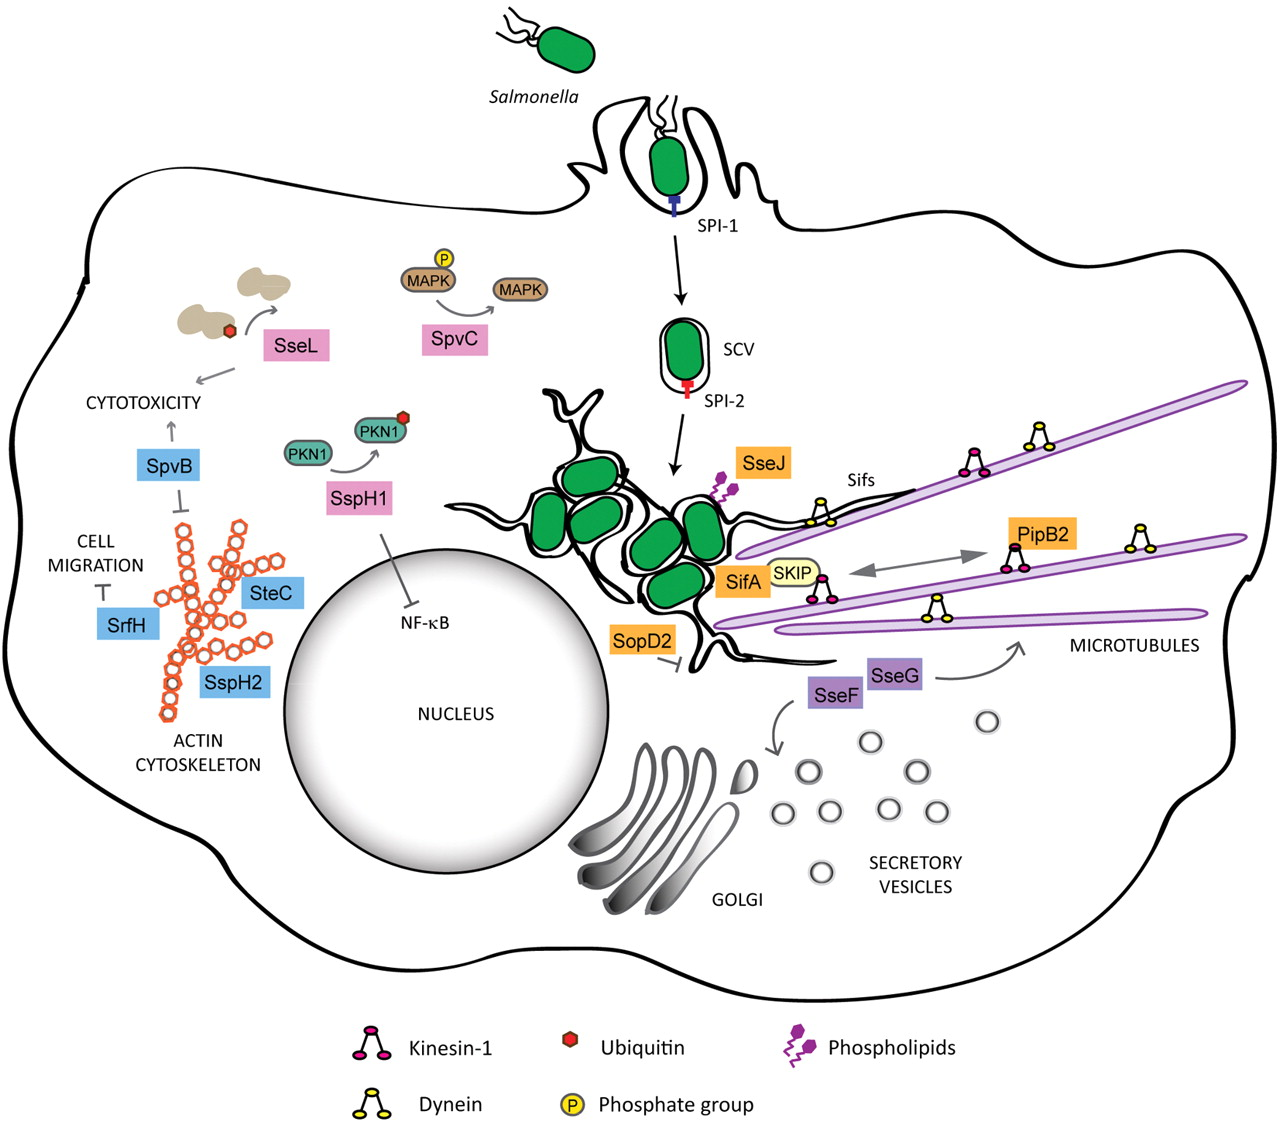
\includegraphics[width=14cm]{SCV.jpg}
\caption[Biogenesis of the \textit{Samonella} containing vacuole]{\textbf{Biogenesis of the \textit{Samonella} containing vacuole (SCV).} \textit{Salmonella} adheres to the outer membrane of host cells, and uses the SPI-1 T3SS and its associated effectors to induce membrane ruffling and entry into the SCV. The SPI-2 T3SS functions mainly in maintenance of the SCV, through the action of the effectors SifA, SopD2, SseJ and PipB2 (orange boxes), and its localization near the Golgi of host cells, mediated by SseF and SseG (purple boxes). Other effectors are involved in modulation of host immune signalling (SpvC, SspH1 and SseL; pink boxes) or target the host cytoskeleton (SteC, SpvB, SspH2 and SrfH; blue boxes). Reproduced from \textcite{Figueira2012} under a Creative Commons Attribution License (CCAL). 
} 
\label{fig:SCV}
\end{center}
\end{figure}

\subsection{Conditional gene fitness}

Determining conditional gene fitness presents a somewhat different problem to that addressed in the previous chapter, predicting and comparing ``essential'' genes under the conditions of library creation. In predicting gene essentiality, we had a single time point representing the initial growth of the library on rich media, while in identifying conditional gene fitness (measured as the relative expansion or contraction of mutant populations) we are always comparing changes in mutant fitness with respect to fitness in a baseline condition. The ratio of reads between the two conditions is taken as indicative of differences in relative mutant prevalences between them. In some ways, this makes the problem of identifying genes with strong fitness effects easier: as we are primarily interested in the ratio of various insertion mutants present between the two conditions, effects that may confound the prediction of simple gene essentiality are effectively ``zeroed out''. More explicitly, whether low insertion density in the initial library occurs due to chance, nucleotide composition bias, or the exclusionary effects of high-density DNA-binding proteins (described in section 2.3.3) does not matter -- these regions can simply be identified as not producing sufficient reads over insertion-sites to be assayed and removed from the analysis.

In many ways, the problem of investigating the statistical and biological significance of ratios of reads over insertion sites resembles established analyses developed for differential RNA-seq analysis. In the following sections I describe the application of these methods to the problem of determining conditional gene fitness.

\section{Experimental methods}
\textit{Gemma C. Langridge performed all laboratory experiments described in this chapter, as well as read mapping; brief descriptions are included here for completeness. Silvia Pinero prepared the THP-1 cells for infection. Sabine Eckert and Daniel Turner performed the nucleotide sequencing. A more detailed description of the experimental methods is available in \textcite{Langridge2010}, including preliminary assessments of bacterial strain ability to grow in RPMI\nomenclature[Z]{RPMI}{Rosewell Park Memorial Institute (cell culture medium)}, invade THP-1 derived macrophage, and experiment optimization.}

\subsection{Strains and cell lines}
These experiments were performed with \textit{S.} Typhi WT174 and  \textit{S.} Typhimurium SL3261 transposon mutant libraries, described in chapter 3. Annotations and orthology predictions used are as in chapter 3. Human monocytic cell line THP-1 was used for cell infections. 

\subsection{Preparation of THP-1 cells}

THP-1 cells were grown up from frozen stocks in RPMI-1640 supplemented with 10\% heat-inactivated foetal bovine serum and 2 mM L-glutamine, and incubated without shaking in vented flasks (VWR, Lutterworth, UK) at 37$^\circ$C in the presence of 5\% CO$_2$. Culture volumes were split and given fresh media every 3-4 days until the desired volume and cell density was achieved. Phorbol myristate acetate (PMA)\nomenclature[Z]{PMA}{Phorbol myristate acetate} was used to differentiate the THP-1 monocytes. Briefly, approximately 212 cells in 4 mL supplemented RPMI containing 0.125 ng/mL PMA were seeded into each well of a 6-well plate and incubated for six days at 37$^\circ$C in 5\% CO$_2$. On the day of infection, the PMA-containing media was removed, cells were washed with dPBS\nomenclature[Z]{PBS}{Phosphate-buffered saline} and fresh warmed, supplemented RPMI was added to maintain the cells while the bacterial inoculum was prepared.

\subsection{Preparation of transposon libraries}

Frozen stocks of the Typhi library were found to be at half the concentration of the Typhimurium library by OD600. To ensure similar concentrations for the infection assay, a 1 in 5000 dilution of the Typhi library and a 1 in 10,000 dilution of the Typhimurium library was used to inoculate the growth medium. Cultures of each transposon library were grown with shaking in 100 mL of RPMI-1640 supplemented with 0.3 g/L L-glutamine and buffered with 10 mL 1 M MOPS at 37$^\circ$C for 16 hours. These cultures were sub-cultured 1 in 20 into fresh RPMI supplemented and buffered as before, and grown for between 3 and 4 hours to mid-log phase (OD600 of 2.4).

\subsection{Infection assay}

Five 6-well plates were used for each run of the assay. In total, 29 wells were infected with the bacterial inoculum and one served as a blank control for eukaryotic cell contamination. At the start of the assay, media was removed from all wells except for the blank control, and a 3 mL bacterial inoculum was added to each experimental well. The plates were centrifuged for 5 minutes at 600 x g and incubated at 37$^\circ$C in 5\% CO$_2$ for 30 minutes. A 4-6 mL aliquot of the inoculum was processed for genomic DNA as the TraDIS control. After 30 minutes, media was removed from all wells, and fresh RPMI additionally supplemented with 100 $\mu$g/mL gentamicin was added. After 2 hours the wells were washed 3 times in plain dPBS. Following washing, 500 $\mu$L of 1\% Triton-X-100 was added to each well to lyse the eukaryotic cells, mixed well by pipetting, and incubated at 37$^\circ$C in 5\% CO$_2$ for 2 minutes. The cell suspensions from all experimental wells were pooled for bacterial DNA extraction. Genomic DNA was extracted using the Qiagen DNeasy Blood and Tissue kit, according to the manufacturer�s protocol for Gram negative bacteria. Sequencing was performed as described in section 2.2.4.

\section{Analysis of conditional gene fitness using TraDIS}

\subsection{Experimental design}

The goal for this experiment was to determine the differences in gene requirements for human macrophage invasion in two \textit{Salmonella} serovars: Typhimurium, a host-generalist, and Typhi, host-restricted to humans as described in the previous chapter. To this end, infection assays of activated THP-1 monocytes were performed in triplicate with transposon libraries for each serovar at high multiplicities of infection in an attempt to avoid bottleneck effects. These were compared to libraries grown in cell culture medium (RPMI), to control for any incidental changes in library composition due to growth in this medium.

\subsection{Mapping insertion sites}

Read mapping is a special case of one of the oldest problems in bioinformatics, aligning a short sequence of length $n$ to a much longer sequence, or database of sequences of length $m$. An optimal solution (with respect to a particular sequence similarity scoring scheme) for this problem using dynamic programming was first proposed by \textcite{Smith1981}, building on previous work by \textcite{Needleman1970}. Unfortunately, this method requires construction of a dynamic programming matrix of size $n \times m$, which quickly becomes impractical for large $m$ due to both time and memory constraints. Heuristic solutions to this problem have been developed, starting with the FASTA and BLAST\nomenclature[Z]{BLAST}{Basic local alignment search tool} algorithms \parencite{Lipman1985,Altschul1990}. The basic idea behind these heuristics is to rapidly search for identical matches using a hash of either the database or query sequence before performing a full Smith-Waterman style local alignment around this match. For the case of mapping reads to larger eukaryotic genomes, more powerful heuristics, such as the Burrows-Wheeler transform \parencite{Burrows1994, Langmead2009, Li2010}, may be required due to time and space constraints. However as we are working with relatively small bacterial genomes, MAQ \parencite{Li2008} has been used here, which is similar in spirit to FASTA or BLAST, but with additional refinements to deal with repetitive genomic regions and to assessing alignment quality.

\subsection{Quality control}

We can asses the quality of TraDIS experiments on multiple levels: the number of reads containing transposon tags and mapping to the genome, the number of insertion sites recovered, the correlation between the numbers of reads recovered for each gene in replicated experiments, and clustering experiments using a dimensionality reduction technique such as principal component analysis (PCA)\nomenclature[Z]{PCA}{Principal component analysis}.

% Table generated by Excel2LaTeX from sheet 'Sheet1'
%
\begin{table}
   \tiny
   \centering
   \noindent
    \caption[Summary statistics for macrophage infection assay sequencing runs]{\textbf{Summary statistics for macrophage infection assay sequencing runs.} Table columns as follows: 1, description; 2, total sequencing reads; 3, reads containing transposon tag; 4, reads mapped to chromosome with quality score greater than 20; 5, number of insertions recovered. STY: \textit{S.} Typhi; STM: \textit{S.} Typhimurium. }
    \begin{tabular}{ l
    				r
				r
				r
				r
				}
   
    \\
     \toprule
    \textbf{Description} & \textbf{Reads} & \textbf{Reads tagged} & \textbf{Reads mapped} & \textbf{Insertion sites} \\
    \midrule
    STY control 1 & 11107014 & 10534361 & 9722100 & 154356\\
    STY control 2 & 10983030 & 10016035 & 8868829 & 193417\\
    STY control 3 & 13506872 & 12168442 & 11062549 & 180998\\
    STY infection 1 & 7526390 & 4193529 & 2304138 & 90218\\
    STY infection 2 & 8630360 & 4166256 & 2000771 & 73154\\
    STY infection 3 & 8215834 & 4323817 & 2459573 & 98894\\
    STM control 1 & 14583559 & 14314003 & 9318191 & 365266\\
    STM control 2 & 18119496 & 17494267 & 11458349 & 464036\\
    STM control 3 & 13565707 & 12457266 & 7312946 & 179702\\
    STM infection 1 &  3292265 & 2972803 & 2033041 & 41775\\
    STM infection 2 & 6444469 & 5351193 & 3732480 & 59476\\
    STM infection 3 & 13012186 & 12124834 & 9633788 & 43110\\
    \bottomrule
    \end{tabular}%
    \label{tab:readmap}%
\end{table}



Summary statistics of the sequencing runs for this study are presented in table \ref{tab:readmap}. Total read yield varied from $\sim$6.4 to $\sim$18.1 million reads, with lower yields generally observed for the infection libraries. Similarly, the percentage of reads containing transposon sequence is significantly lower in the {\it S.} Typhi infection samples. However, despite these issues, over two million reads over insertion sites were recovered in every sample which provides adequate coverage for this assay. Interestingly, the number of unique insertion sites recovered from the {\it S.} Typhimurium infection assays was approximately half that observed in the {\it S.} Typhi assay in every replicate, despite having an apparently more complex inoculum. This is suggestive of either stronger selective pressure, a more severe bottleneck effect, or both for {\it S.} Typhimurium compared to {\it S.} Typhi during infection of human macrophage, as might be expected given the latter's host adaptation.

Linear correlation coefficients, reported in table \ref{tab:pear} lend some credence to this idea that {\it S.} Typhimurium may be experiencing a more severe bottleneck leading to the incidental loss of mutants during infection, possibly due to the killing effects of the macrophage. Correlations between replicate experiments are over .99 with two notable exceptions. The first is in the third replicate of the {\it S.} Typhimurium assay. Due to failure of this replicate during the current study, an earlier 2 hour time point from optimization experiments \parencite{Langridge2010} was used, so the lower correlation between the third control replicate and replicates 1 and 2 may be explained by this sample being handled at a different time and sequenced earlier on a different machine. However, the correlation coefficient between the third control replicate and replicates 1 and 2 is still well over .9, indicating that it still largely agrees with the later experiments.

% Table generated by Excel2LaTeX from sheet 'Sheet1'
%
\begin{table}
   \tiny
   \centering
   \noindent
    \caption[Pearson's {\it r} between replicated TraDIS experiments]{\textbf{Pearson's {\it r} between replicated TraDIS experiments.} Correlations of reads over genic and non-coding RNA features between replicated control and infection assays. Y: \textit{S.} Typhi; M: \textit{S.} Typhimurium; C: Control; I: Infection. }
    \begin{tabular}{ l
    				l
				l
				l
				l
				l
				l
				l
				l
				l
				l
				l
				l
				}
   
    \\
     \toprule
    &\textbf{Y C1} & \textbf{Y C2} & \textbf{Y C3} & \textbf{Y I1} & \textbf{Y I2} & \textbf{Y I3} &  \textbf{M C1}&  \textbf{M C2} &  \textbf{M C3} &  \textbf{M I1}&  \textbf{M I2}&  \textbf{M I3}\\
    \midrule
\textbf{Y C1} &   1.00 & 0.99 & 0.99 & 0.65 & 0.69 & 0.72 & 0.43 & 0.43 & 0.48 & 0.34 & 0.39 & 0.43\\
\textbf{Y C2} &  0.99 & 1.00 & 0.99 & 0.65 & 0.70 & 0.72 & 0.42 & 0.43 & 0.48 & 0.33 & 0.39 & 0.43\\
 \textbf{Y C3} & 0.99 & 0.99 & 1.00 & 0.67 & 0.71 & 0.74 & 0.44 & 0.44 & 0.49 & 0.34 & 0.40 & 0.45\\
 \textbf{Y I1} & 0.65 & 0.65 & 0.67 & 1.00 & 0.99 & 0.99 & 0.26 & 0.28 & 0.32 & 0.30 & 0.31 & 0.49\\
\textbf{Y I2} &  0.69 & 0.70 & 0.71 & 0.99 & 1.00 & 0.99 & 0.28 & 0.28 & 0.34 & 0.31 & 0.33 & 0.49\\
  \textbf{Y I3} & 0.72 & 0.72 & 0.74 & 0.99 & 0.99 & 1.00 & 0.29 & 0.29 & 0.35 & 0.31 & 0.33 & 0.50\\
 \textbf{M C1}&  0.43 & 0.42 & 0.44 & 0.26 & 0.28 & 0.29 & 1.00 & 0.99 & 0.93 & 0.74 & 0.85 & 0.76\\
\textbf{M C2}&  0.43 & 0.43 & 0.44 & 0.26 & 0.28 & 0.29 & 0.99 & 1.00 & 0.93 & 0.73 & 0.85 & 0.77\\
 \textbf{M C3} &  0.48 & 0.48 & 0.49 & 0.32 & 0.34 & 0.35 & 0.93 & 0.93 & 1.00 & 0.69 & 0.80 & 0.75\\
 \textbf{M I1} & 0.34 & 0.33 & 0.34 & 0.30 & 0.31 & 0.31 & 0.74 & 0.73 & 0.69 & 1.00 & 0.74 & 0.68\\
  \textbf{M I2} & 0.39 & 0.39 & 0.40 & 0.31 & 0.33 & 0.31 & 0.85 & 0.85 & 0.80 & 0.74 & 1.00 & 0.72\\
 \textbf{M I3} &  0.43 & 0.43 & 0.45 & 0.49 & 0.49 & 0.50 & 0.76 & 0.75 & 0.75 & 0.68 & 0.72 & 1.00\\
    \bottomrule
    \end{tabular}%
    \label{tab:pear}%
\end{table}



The other discrepancy is in the correlation between {\it S.} Typhimurium infection experiments, with coefficients ranging between .68 and .74. This is still a high positive correlation, however it does not reach the level observed in the other replicated experiments in this study. This is again suggestive of a bottleneck effect in this assay. If the loss of particular mutants were purely due to selection, we would expect a high correlation, as these losses would presumably be reproducible under the same experimental conditions. Rather, it appears that there is some stochasticity in the loss of mutants in this particular experiment, suggesting losses that are incidental to the actual factors underlying infection of human macrophage. As mentioned previously, this may be due to a higher rate of macrophage killing of the non-host adapted {\it S.} Typhimurium strain used in this study. It has been observed previously that even in {\it S.} Typhimurium strains capable of successfully infecting macrophage, some proportion of the invading bacteria do not manage to establish a protective SCV \parencite{Monack1996} for reasons that remain unclear. A higher rate of failure in establishing the SCV in human macrophage for {\it S.} Typhimurium than {\it S.} Typhi, or even the use of an entirely different mechanism for survival in macrophage by {\it S.} Typhi, may explain this difference.

\begin{figure}[htp]
\begin{center}
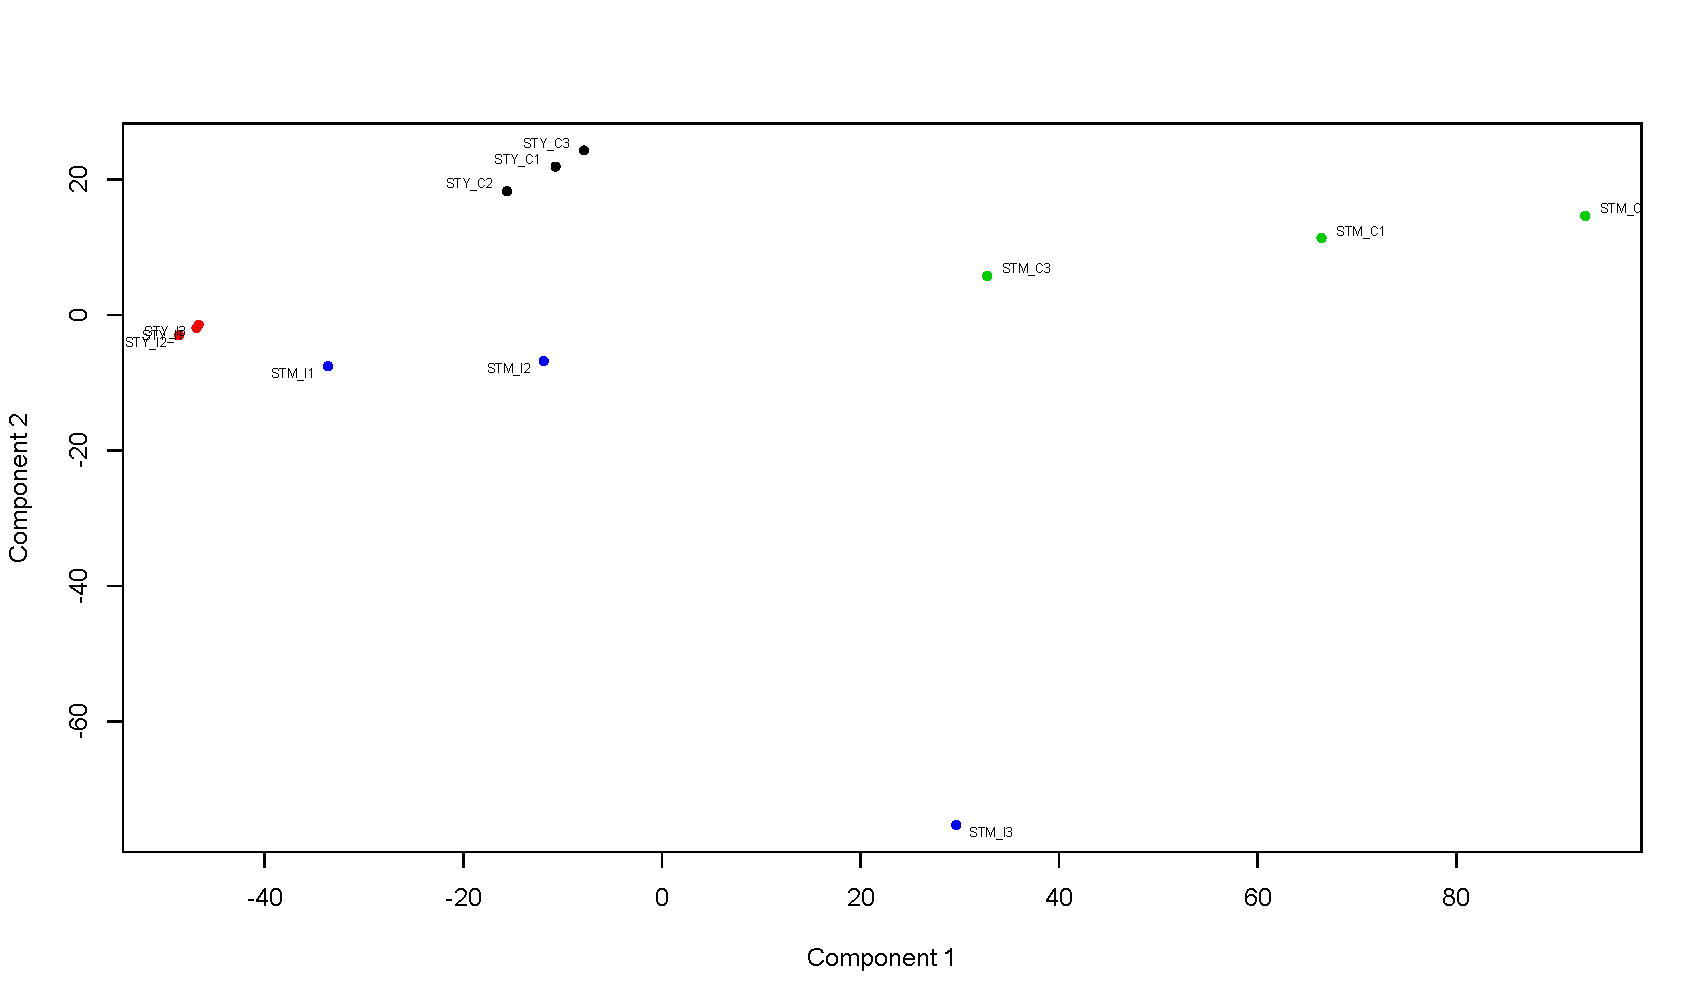
\includegraphics[width=14cm]{PCA}
\caption[Principal component analysis of TraDIS macrophage infection assays]{\textbf{Principal component analysis of TraDIS macrophage infection assays.} Plot showing samples along first two components of a PCA, representing 55\% and 18\% of the total variance in the data set, respectively. Replicates appear to cluster together, with the exception of the third Typhimurium infection replicate, which was excluded from the analysis. STY: {\it S.} Typhi; STM: {\it S.} Typhimurium; C: control; I: infection. 
} 
\label{fig:PCA}
\end{center}
\end{figure}

To further investigate the potential bottleneck effect in {\it S.} Typhimurium, I performed a principal component analysis (PCA) on all samples. PCA is a mathematical technique for dimensional reduction which identifies linear vectors (components) in a high-dimensional dataset which capture maximal amounts of the variance between samples. This high dimensional data can then be visualized in a lower (e.g. 2 or 3) dimensional space by plotting samples against these components. Samples were centered and scaled to correct for the differences in read counts between experiments. Plots of all samples in this study on the first two principal components, accounting for 55\% and 18\% of the total variance respectively, are shown in figure \ref{fig:PCA}. With the exception of the third {\it S.} Typhimurium infection experiment, all samples collected under the same conditions cluster on this plot, as would be expected if these results are reporting the effects of differential selection. All infection samples lie to the left of their respective control samples on the first component, suggesting that the dominant signal in this data is due to the effects of selection during macrophage infection. The fact that two of the three {\it S.} Typhimurium infection experiments cluster together suggests that this signal is stronger than any stochastic bottleneck effect despite the lower correlations observed between these libraries, and that it should be possible to derive useful information about the conditions faced by {\it S.} Typhimurium during infection from these experiments. Unfortunately, the third {\it S.} Typhimurium infection replicate, which was performed separately as described earlier, does not cluster well with these. I performed a similar analysis using the plotMDS function of edgeR \parencite{Robinson2010}, which performs multidimensional scaling using a variance-stabilized distance measure between samples, and came to a similar result. It is unclear why this is the case, and it may be due to differences in experimental set up or sequencing. I excluded this replicate from further analysis on this basis.

\subsection{Inter-library normalization}

Normalization is a critical part of any high-throughput sequencing experiment. As observed in the previous section, even the same experiment repeated on the same machine can lead to very different read counts. The naive approach to solving this problem is simply to scale each sequencing library by some factor so that the total read counts are equivalent. This may be adequate for analysis of technical replicates where gene expression levels are identical between all samples. However, \textcite{Robinson2010a} illustrate why this may not be the case for the comparison of sequencing libraries sampling populations under different conditions with a simple thought experiment:

\begin{quote}
Imagine we have a sequencing experiment comparing two RNA populations, A and B. In this hypothetical scenario, suppose every gene that is expressed in B is expressed in A with the same number of transcripts. However, assume that sample A also contains a set of genes equal in number and expression that are not expressed in B. Thus, sample A has twice as many total expressed genes as sample B, that is, its RNA production is twice the size of sample B. Suppose that each sample is then sequenced to the same depth. Without any additional adjustment, a gene expressed in both samples will have, on average, half the number of reads from sample A, since the reads are spread over twice as many genes. Therefore, the correct normalization would adjust sample A by a factor of 2. \parencite{Robinson2010a}
\end{quote}

More generally, we can think of each gene in a sequencing library as representing a slice of a pie. If a particular gene increases in expression (or mutant prevalence for transposon-insertion sequencing such as ours), then the space left in this pie for other genes necessarily shrinks. A scaling normalization which does not take this fact in to account, but simply assumes all pies are the same size would necessarily underestimate expression (or prevalence) for the majority of genes which don't change, while overestimating it for the few that do. A recent study has shown that normalization methods which explicitly account for this problem perform better on both real and simulated data \parencite{Dillies2012}. Here I have used the trimmed mean of M-values (TMM)\nomenclature[Z]{TMM}{Trimmed mean of M-values} method, which assumes the majority of genomic features do not change in actual expression (or mutant prevalence here) and attempts to align the read counts of these features to produce an appropriate scaling factor \parencite{Robinson2010a}.

\subsection{Identifying fitness effects}

\subsubsection{Theory}
Once sequencing libraries have been normalized, the next step in determining fitness effects is the choice of a proper test to determine the significance of changes in read counts. In the previous chapter, I used two test statistics. The first was to test for gene requirements within a particular library, and this was accomplished by fitting gamma distributions to the two modes observed in the empirical distributions of insertion indexes, then setting a threshold based on a log-odds ratio (see figure \ref{fig:gamma}). The second was to additional test for significant differences in read depth between the {\it S.} Typhimurium and {\it S.} Typhi libraries. In this case the $log_2$ read ratios between genomic features in the two libraries were roughly normally distributed, and I was able to set a significance threshold based on a fitted normal curve.

Neither of these tests are entirely appropriate for the present situation of identifying reproducible changes in mutant prevalence in replicated experiments. Most obviously, neither of these test can easily be modified to accommodate replicates, which is essential for robust identification of changes in mutant prevalence. Secondly, both tests are dependent on manual fitting of gamma or normal distributions, which can not easily or robustly be automated. Standard statistical tests, such as the two sample Student's T-test or Mann-Whitney U-test are not applicable due to the small numbers of replicates (3 here, often 2) because of high experimental overhead in replication. Fortunately, these problems have largely been addressed in modern RNA-seq differential expression analysis software.

The two leading packages for analysis of RNA-seq based differential expression analysis are DESeq \parencite{Anders2010} and edgeR \parencite{Robinson2010}. Both assume that sequence count data is negative binomially distributed. The negative binomial distribution arises naturally in the case of a Poisson process sampling from gamma-distributed random variables \parencite{Fisher1941}. Sequencing of mixed populations of oligonucleotides has long been theorized to behave as a Poisson process, and this has shown to roughly be the case for technical replicates of Illumina RNA-seq runs \parencite{Marioni2008}, i.e. repeated sequencing of the same input sample. Other studies have shown that biological RNA-seq and SAGE\nomenclature[Z]{SAGE}{Serial analysis of gene expression} replicates, i.e. repeated experiments, generate extra-Poisson variability \parencite{Lu2005, Robinson2007}, possibly due to variability in the concentration of the transcripts being sampled, which can be captured by the negative binomial.

This leads naturally to the question, is transposon-insertion sequencing data negative binomially distributed? Obviously, technical replicates of TraDIS experiments will be roughly Poisson distributed, as this is identical to the case of technical replication of RNA-seq. The question then becomes whether the underlying distribution of mutant prevalences being sampled by sequencing can be effectively modelled by a gamma distribution. Theoretical considerations indicate that this model may be appropriate: as subcultures of the mutant library expand, the number of insertion mutants per gene will be the summed result of independent exponentially-expanding clones, which will be gamma distributed assuming the starting populations are roughly equal. The only way to answer this question definitively would be to repeat the same experiment a large number of times, which is impractical. However, this is not necessary. \textcite{Lu2005} showed that the negative binomial assumption is highly robust to the actual distribution of the data being assessed. In fact, it appears that the underlying transcript prevalences being sampled by RNA-seq experiments may actually be distributed according to a sum of log-normal distributions \parencite{Bengtsson2005}; this does not prevent DESeq and edgeR from performing competitively in benchmarks of differential expression analysis \parencite{Kvam2012, Soneson2013}. These approaches have previously been successfully applied to other Illumina sequencing-based experiments which likely have different underlying distributions than transcriptomic data, for instance differential analysis of ChIP-seq\nomenclature[Z]{ChIP-seq}{Chromatin immunoprecipitation sequencing} data \parencite{Robinson2012}.

I have used edgeR \parencite{Robinson2010} for significance testing here, a R package which implements the TMM normalization  \parencite{Robinson2010a}, an approximation to an empirical Bayes estimation of feature-wise negative binomial dispersion parameters \parencite{Robinson2007}, and a version of Fisher's exact test modified to deal with overdispersed data \parencite{Robinson2008} as well as a likelihood-ratio test in the case of multifactorial designs \parencite{McCarthy2012, Lund2012}. After testing, we are interested primarily in two values: the P-value given by the statistical testing which tells us how confident we can be that mutant prevalence differs between two conditions given the estimated negative binomial distribution distribution of read counts, and the $log_2$ fold-change (logFC\nomenclature[Z]{logFC}{$Log_2$ fold-change}) which gives an estimation of the magnitude of the difference. LogFC is calculated as \[ logFC_g = log(n_{g,b}) - log(n_{g,a})\] where the index $g$ indicates the genomic feature being tested, $n_{g,b}$ is the normalized average read count in the test condition, and $n_{g,a}$ is the normalized average read count in the control condition. This subtraction is equivalent to taking the $log$ of the ratio $\frac{n_{g,b}}{n_{g,a}}$, and hence $logFC_g$ becomes unstable for small changes in $n_{g,b}$ as $n_{g,a} \to 0$, and is ultimately undefined when $n_{g,a} = 0$. In the previous chapter I corrected for this by adding a pseudocount to each gene's read count. I take the same approach here, as implemented in edgeR, only since each library has been normalized by a different factor, I rather use the transformation \[ n^T_{g,x} = log(\frac{n_{g,x}}{L_x} + \frac{2}{ \overline{L}})\] where $L$ is the library size. This has the effect of shrinking unreliable logFCs for features with small read counts, and removing the problem of undefined logFCs.

\subsubsection{Application to macrophage infection data}

Returning to the macrophage infection assays, I first eliminated genomic features from consideration which did not have at least 20 counts per million normalized reads (CPM\nomenclature[Z]{CPM}{Counts per million (reads)}) in at least three assay or control replicates. This cut-off is arbitrary, but serves the purpose of removing features from consideration which do not have adequate read coverage to deliver biologically significant results in at least one condition. This provides two advantages: firstly, it increases statistical power by reducing the number of simultaneous hypothesis tests that need to be corrected for, and secondly, it eliminates features which may have statistically significant logFCs but may not have large enough mutant populations to determine if these effects are biologically relevant. This reduces the number of genomic features tested from 3882 (including all orthologous coding sequences and non-coding RNAs) to 3596.

I then set up three statistical analyses within the generalized linear model (GLM\nomenclature[Z]{GLM}{Generalized linear model}) framework provided by edgeR, which allows for multi-factorial analyses. The first tests whether the logFC between {\it S.} Typhimurium infection and control is different from the logFC between {\it S.} Typhi infection and control. This allows me to discriminate between mutant populations which behave similarly during macrophage invasion in the two serovars (no or small difference in logFCs), from those which behave differently (large difference in logFCs). Of course, this does not allow me to discriminate between mutant populations which are expanding, those that are shrinking, or those which are static in both serovars during invasion - this test only tells if their behavior is similar. Similarly, using this test I can not discriminate between features with differences in logFCs that are the result of mutant expansion in one serovar, or contraction in another. For this reason I performed two additional analyses, testing the significance of logFCs between infection and control in each serovar independently. All p-values have been corrected for multiple testing using the method of \textcite{Benjamini1995}, controlling for a false discovery rate (FDR\nomenclature[Z]{FDR}{False discovery rate}) of 10\%.

\begin{figure}[htp]
\begin{center}
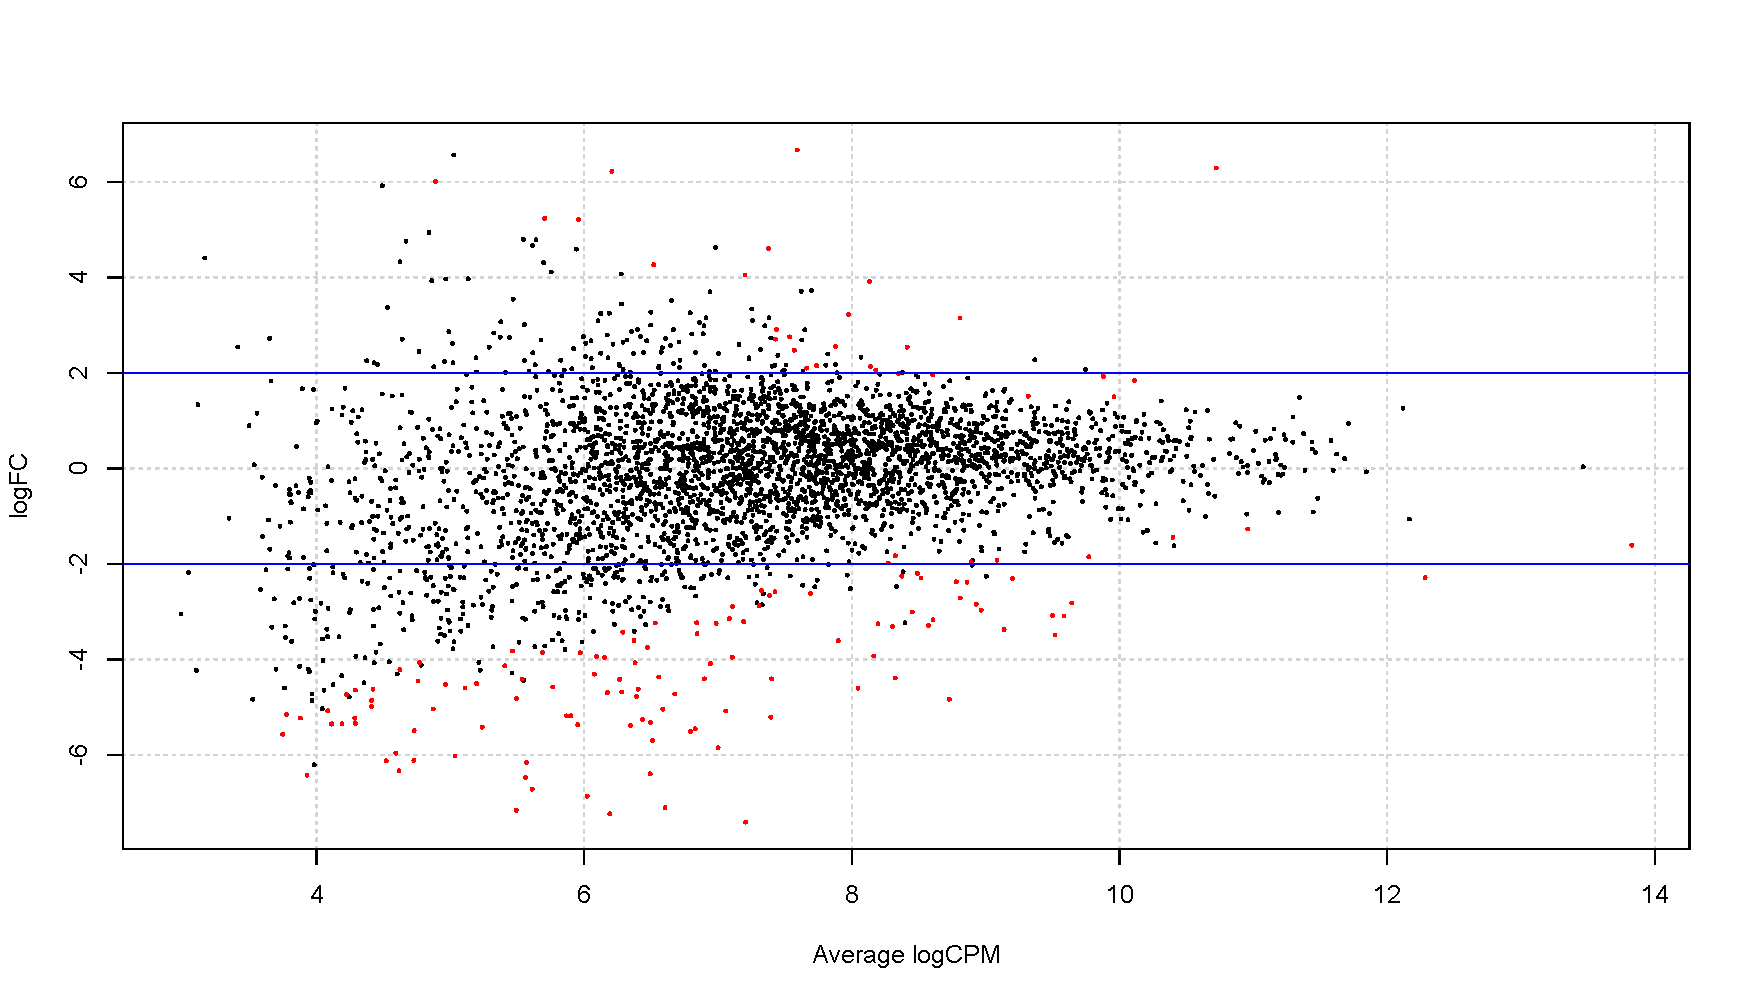
\includegraphics[width=14cm]{STMvTY}
\caption[Smear plot of differences in logFC over macrophage infection between {\it S.} Typhimurium and {\it S.} Typhi]{\textbf{Smear plot of differences in logFC over macrophage infection between {\it S.} Typhimurium and {\it S.} Typhi.} Each point in this plot represents a tested genomic feature. LogFC is reported on the Y-axis, logCPM on the X-axis; statistically significant features at a FDR of 0.1 are in red. The blue lines represent logFCs of $|2|$, translating to a four-fold difference in logFC in mutant prevalences between the two serovars.
} 
\label{fig:svt}
\end{center}
\end{figure}

\begin{figure}[htp]
\begin{center}
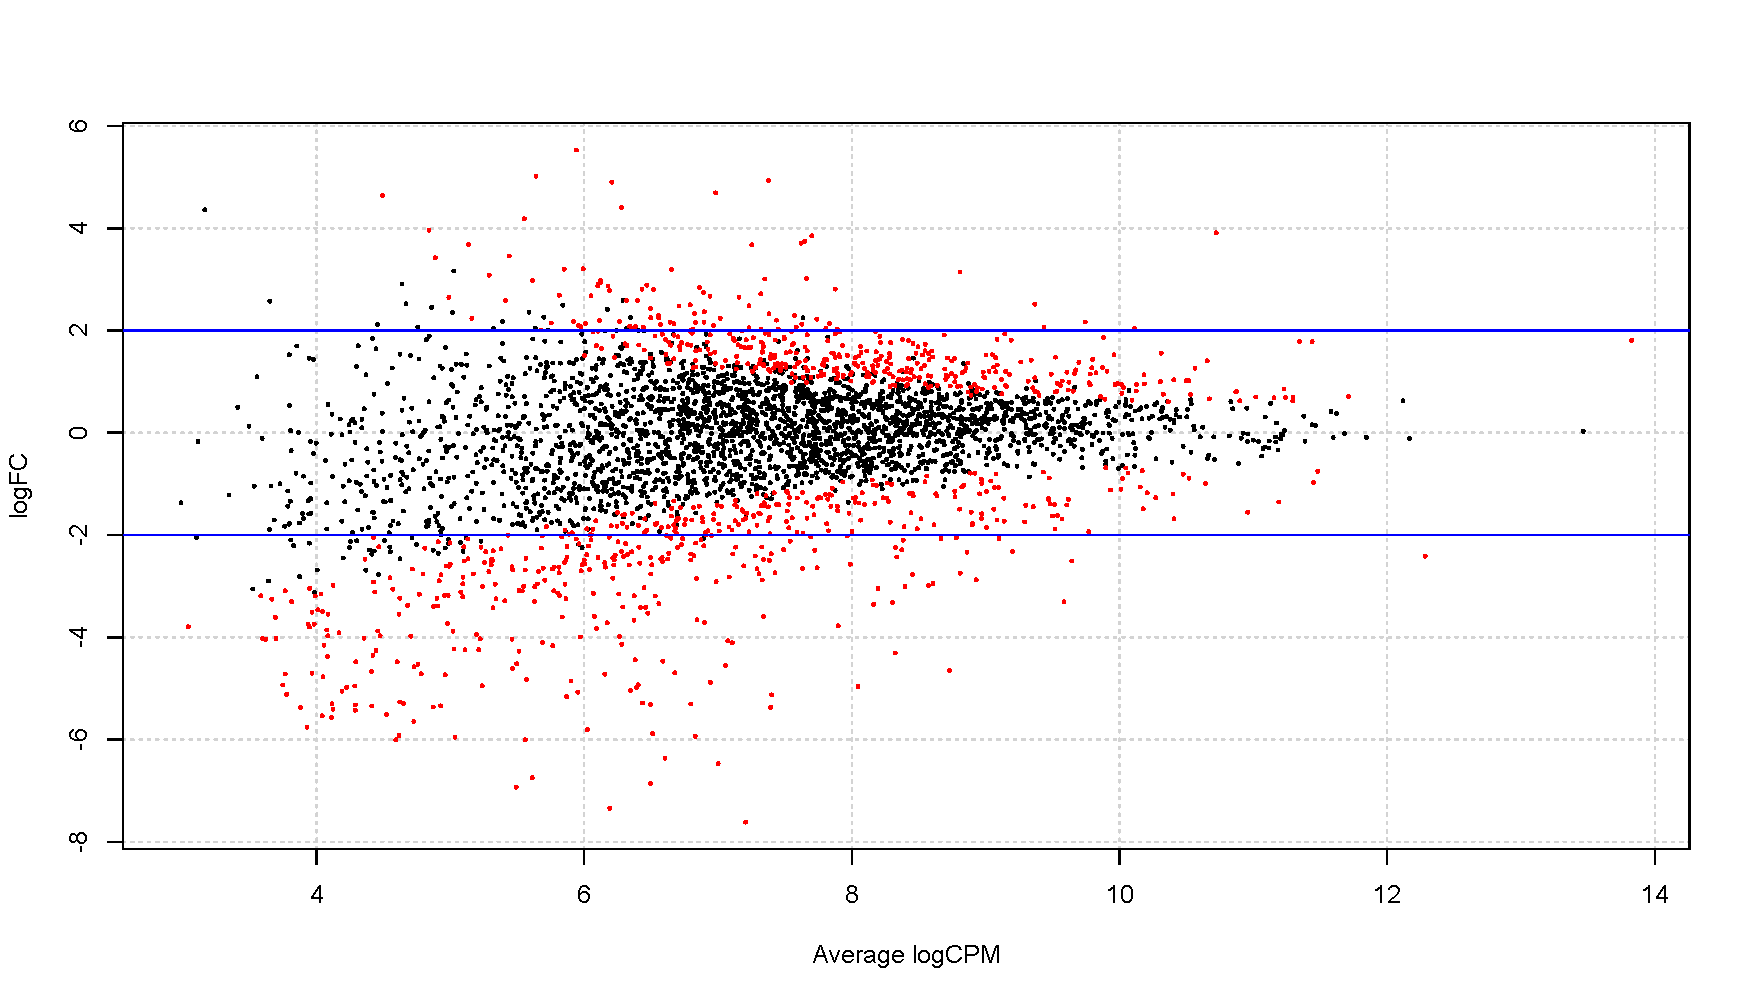
\includegraphics[width=14cm]{STM}
\caption[Smear plot of logFC in mutant prevalences over macrophage infection in {\it S.} Typhimurium]{\textbf{Smear plot of logFC in mutant prevalences over macrophage infection in {\it S.} Typhimurium.} Each point in this plot represents a tested genomic feature. LogFC is reported on the Y-axis, logCPM on the X-axis; statistically significant features at a FDR of 0.1 are in red. The blue lines represent logFCs of $|2|$, translating to a four-fold change in mutant prevalences between infection and control.
} 
\label{fig:stm}
\end{center}
\end{figure}

\begin{figure}[htp]
\begin{center}
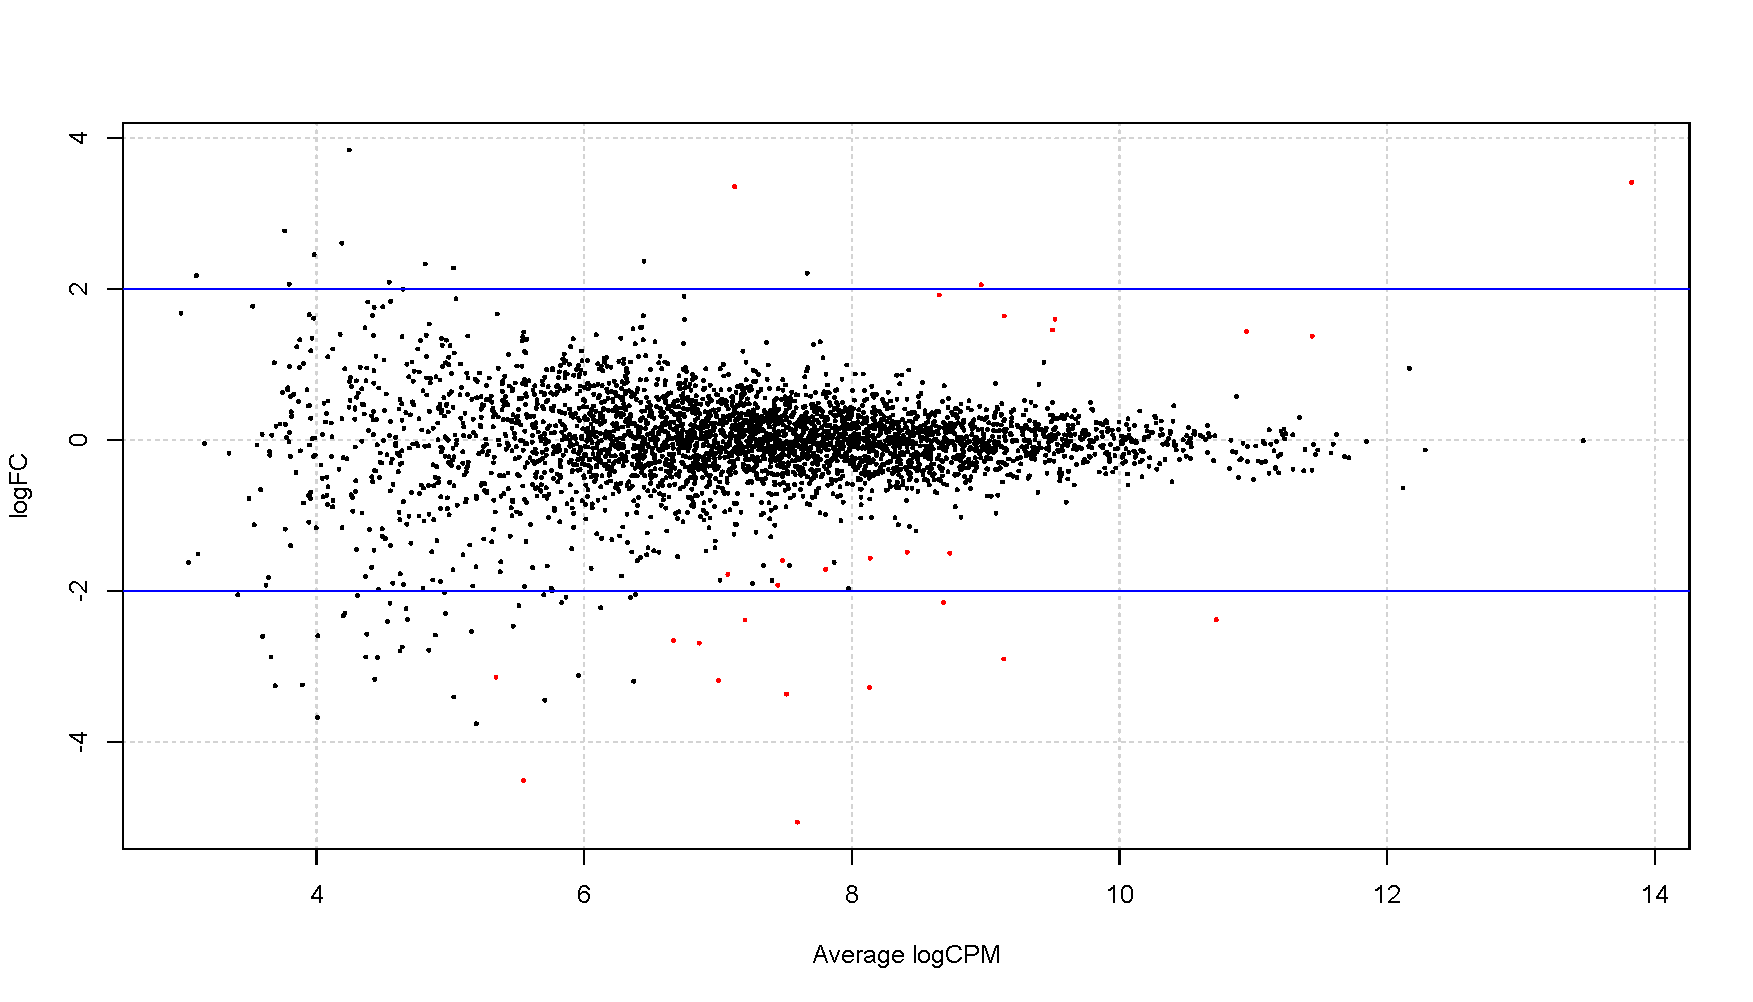
\includegraphics[width=14cm]{TY}
\caption[Smear plot of logFC in mutant prevalences over macrophage infection in {\it S.} Typhi]{\textbf{Smear plot of logFC in mutant prevalences over macrophage infection in {\it S.} Typhi.} Each point in this plot represents a tested genomic feature. LogFC is reported on the Y-axis, logCPM on the X-axis; statistically significant features at a FDR of 0.1 are in red. The blue lines represent logFCs of $|2|$, translating to a four-fold change in mutant prevalences between infection and control.
} 
\label{fig:TY}
\end{center}
\end{figure}

The results of the comparison between {\it S.} Typhimurium and {\it S.} Typhi changes in logFC over macrophage infection are shown in figure \ref{fig:svt}, and the individual changes in mutant prevalences for each serovar are shown in figures \ref{fig:stm} and \ref{fig:TY}. On first viewing these figures, there is a striking in the behavior of the {\it S.} Typhimurium and {\it S.} Typhi mutant libraries: while {\it S.} Typhimurium displays a wide spread of changes in mutant prevalence, 938 of them statistically significant, indicating a strong selective pressure operating on the library, the composition of the {\it S.} Typhi library appears nearly unchanged after passaging, with only 28 features showing a statistically significant change in mutant prevalence. In fact it appears that nearly all of the statistically significant differences in logFC between the two libraries over macrophage infection are due to changes in mutant prevalences in the {\it S.} Typhimurium library. This seems to indicate, on a gross level, that {\it S.} Typhi is somehow avoiding the brunt of the gauntlet imposed on {\it S.} Typhimurium in the first two hours of macrophage infection. This may partially be due to the presence of the Vi capsule on {\it S.} Typhi, which has previously been shown to enhance survival in THP-1 derived macrophage \parencite{Hirose1997} though the creation of a `stealth' phenotype which reduces the expression of inflammatory factors, such as TNF-$\alpha$\nomenclature{TNF-$\alpha$}{Tumor necrosis factor $\alpha$}, by the macrophage.

\subsection{Functional analysis of gene sets that affect fitness}

\subsection{Results}

\subsection{Other applications}